\chapter{Production Deployment Details}
\label{appendix:docker}

This appendix details how \textbf{Sensae Console} and the \textbf{Business Applications} are currently managed in production. 

\section{Containerization of services via Docker}
\label{subsec:implementation:decisions:docker}

This section describes how the final product is packaged into containers.

As stated in \citetitleyear{dockerinit}, Docker acts as an intermediary layer between the application to be deployed and the operating system where it will be deployed, ensuring that the developed software has the same behavior regardless of the system. The dependencies of the solution do not have to be present in the system, it is only necessary to install the Docker tool in the \gls{OS}.

This tool thus makes it possible to lower the coupling between the \gls{OS} and the software to be deployed.

With regards for this solution, each container defined in Section~\ref{sec:design:architecture} is mapped into a docker container.
A container is often compared to a virtual machine running on a hypervisor or \gls{OS}, but it has a much lower resource consumption, since only the application runs and not not all the processes inherent to an \gls{OS} as described by \cite{bernstein2014containers}.

The Figure~\ref{fig:implementation:decisions:docker:contvsvm} compares a \gls{VM} and Container-based deployments.

\begin{figure}[H]
    \centering
    \resizebox{0.7\columnwidth}{!}
    {
       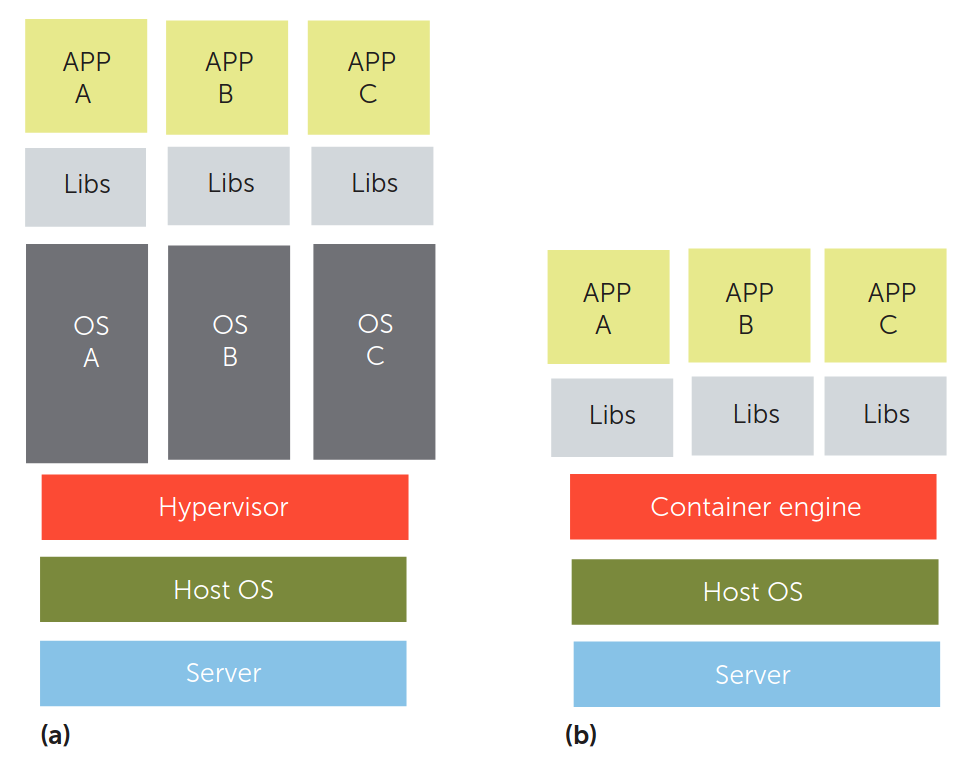
\includegraphics{assets/figures/vmvscontainer.png}
    }
    \caption[Comparison of VM and Container-based deployments]{Comparison of VM (a) and Container-based (b) deployments by \cite{bernstein2014containers}}
    \label{fig:implementation:decisions:docker:contvsvm}
\end{figure}

The system is thus represented as a collection of containers that communicate with each other and the outside through standard protocols such as HTTP or \gls{AMQP}.

The production environment can thus be quickly replicated on another machine in case of a failure disaster or a overwhelming number of interaction with the server.

Details about service containerization can be found in Section~\ref{subsec:implementation:description:docker}.

\section{Orchestration of services via Docker Compose}
\label{subsec:implementation:decisions:compose}

This section describes how the final product is orchestrated using Docker Compose.

As stated in the article \citetitleyear{dockercompose}, ``Compose is a tool for defining and running multi-container Docker applications''.

Currently a single node is capable of handling the traffic generated by all the managed devices and costumers. Due to this, it was decided to use a docker compose in production inserted of tools like Kubernetes (that can ease the process of autoscaling individual containers).

The solution's orchestration is defined in a \textit{YAML} file and then started with a single command. To improve security, only the needed container ports are exposed. To ensure data integrity throughout service disruptions, persistence data is mapped to folder in the \gls{OS}. To ensure an easy management of the environment, configurations are kept in the \gls{OS} and fetched by each container once they start.

The details about the solution orchestration can be found in Section~\ref{subsec:implementation:description:compose}.

\section{Usage of Nginx as a web server and reverse proxy}
\label{subsec:implementation:decisions:nginx}

To serve the frontend pages and redirect requests made to backend containers, the following technologies were analyzed:

\begin{itemize}
    \item \citetitle{nginx};
    \item \citetitle{apachehttp};
    \item \citetitle{lighttpd}.
\end{itemize}

All of them support the necessary requirements, but some factors lead the author to pick Nginx over the others, the following table, Table~\ref{tab:implementation:decisions:nginx:compare}, describes this criteria.

\begin{table}[H]
    \caption{Technologies Comparison - Reverse Proxy Web Server}
    \label{tab:implementation:decisions:nginx:compare}
    \centering
    \begin{tabular}{@{}clll@{}}
    \toprule
    \textbf{Criteria/Technology} & \textbf{Nginx} & \textbf{Apache HTTP Server} & \textbf{Lighttpd} \\ \midrule
    Resource Consumption      & low  & high      & medium \\ \midrule
    Community Size            & high & very high & medium \\ \midrule
    Familiarity with the tool & high & low       & low    \\ \bottomrule
    \end{tabular}
\end{table}

The details about \citetitle{nginx} adoption and configuration can be found in Section~\ref{subsec:implementation:description:nginx}.

\section{Sensae Console Containerization}
\label{subsec:implementation:description:docker}

The section describes how \textbf{Sensae Console} is containerized with docker.
As explained in Section~\ref{subsec:implementation:decisions:docker}, the author choose to containerize the solution.

The following Code Samples describe how each container mentioned during the Design Chapter are packaged. To simplify, only three distinct samples will be presented.

The first sample, Listing~\ref{code:implementation:description:docker:frontend}, refers to UI Aggregator and is similar to all other frontend containers.

\begin{lstlisting}[caption=Dockerfile for UI Aggregator Frontend, label={code:implementation:description:docker:frontend}]
FROM node:18-alpine AS build
WORKDIR /workspace
COPY package.json ./
COPY . .
RUN npm install
RUN npm run nx build ui-aggregator --omit=dev

FROM nginx:1.23.1
COPY apps/ui-aggregator/nginx/nginx.conf /etc/nginx/conf.d/default.conf
COPY --from=build /workspace/dist/apps/ui-aggregator /usr/share/nginx/html
\end{lstlisting}

This Dockerfile contains two stages to reduce the size of the final image. The first stage, lines \textbf{1} to \textbf{6}, builds the project. The second one, containing only \citetitle{nginx} and the code that was previously built, is used to serve the UI Aggregator Frontend and route requests. The \citetitle{nginx} configuration file at line \textbf{9} is discussed in the \ref{subsec:implementation:description:nginx} Section.

The second sample, Listing~\ref{code:implementation:description:docker:spring}, refers to \textbf{Fleet Management Backend} and is similar to all backend containers in the Configuration Scope or Business Applications.

\begin{lstlisting}[caption=Dockerfile for Fleet Management Backend, label={code:implementation:description:docker:spring}]
FROM maven:3.8.5-openjdk-18 AS build
WORKDIR /app
# copy all pom.xml to pull only external dependencies
COPY application/pom.xml application/pom.xml
COPY domain/pom.xml domain/pom.xml
COPY infrastructure/boot/pom.xml infrastructure/boot/pom.xml
COPY infrastructure/endpoint/pom.xml infrastructure/endpoint/pom.xml
COPY infrastructure/persistence/pom.xml infrastructure/persistence/pom.xml
COPY infrastructure/persistence/questdb/pom.xml infrastructure/persistence/questdb/pom.xml
COPY infrastructure/endpoint/graphql/pom.xml infrastructure/endpoint/graphql/pom.xml
COPY infrastructure/endpoint/amqp/pom.xml infrastructure/endpoint/amqp/pom.xml
COPY infrastructure/pom.xml infrastructure/pom.xml
COPY pom.xml pom.xml
# build all external dependencies
RUN mvn -B -e -C org.apache.maven.plugins:maven-dependency-plugin:3.1.2:go-offline -DexcludeArtifactIds=fleet-management-backend,application,domain,infrastructure,endpoint,graphql,boot,amqp,questdb

COPY . .
RUN mvn clean package

FROM openjdk:17
WORKDIR /app
COPY --from=build /app/infrastructure/boot/target/fleet-management-backend.war /app
CMD ["java", "-jar", "fleet-management-backend.war"]
\end{lstlisting}

This sample also presents a multi-stage Dockerfile. The first stage, line \textbf{1} to \textbf{18} builds the project with Maven. All \textit{pom.xml} files and dependencies are added first to reduce build time during development, since these change less that the code written. The second stage is the one that runs the  service. It only contains the \gls{JDK} and the compiled application.

The third sample, Listing~\ref{code:implementation:description:docker:quarkus}, refers to \textbf{Device Commander} and is similar to all backend containers in the Data Flow Scope.

\begin{lstlisting}[caption=Dockerfile for Device Commander, label={code:implementation:description:docker:quarkus}]
FROM quay.io/quarkus/ubi-quarkus-native-image:22.1-java17 AS build
COPY --chown=quarkus:quarkus mvnw /code/mvnw
COPY --chown=quarkus:quarkus .mvn /code/.mvn
COPY --chown=quarkus:quarkus pom.xml /code/
USER quarkus
WORKDIR /code
RUN ./mvnw -B org.apache.maven.plugins:maven-dependency-plugin:3.1.2:go-offline
COPY src /code/src
RUN ./mvnw package -Pnative

FROM quay.io/quarkus/quarkus-micro-image:1.0
WORKDIR /work/
COPY --from=build /code/target/runner /work/application

# set up permissions for user `1001`
RUN chmod 775 /work /work/application \
    && chown -R 1001 /work \
    && chmod -R "g+rwX" /work \
    && chown -R 1001:root /work

EXPOSE 8080
USER 1001

CMD ["./application", "-Dquarkus.http.host=0.0.0.0"]
\end{lstlisting}

This sample, once again, is also a multi-stage Dockerfile. It was adapted from the one generated by \citetitle{quarkus} when setting up the application. In the first stage the application is built with a \citetitle{graalvm} native-image - lines \textbf{1} to \textbf{9}. This allows the image to run without \gls{JVM}. The second stage runs the service after setting user permissions, so that the process doesn't run as root, at lines \textbf{17} to \textbf{20}.

\section{Sensae Console Orchestration}
\label{subsec:implementation:description:compose}

As described in Section~\ref{par:design:architecture:platform:container:physical}, \citetitle{dockercompose} was the tool used to orchestrate the whole solution, the \textbf{Sensae Console} and Business Applications. This tool consumes a configuration file to know what containers, and their configurations, are needed. The complete configuration file for production is vast, a summarized version will be presented containing only the \textbf{Data Processor} Context' related containers.

\begin{lstlisting}[style=yaml, caption=Docker Compose Configuration File for Production, label={code:implementation:description:compose:file}]
services:
  data-processor-frontend:
    build:
      dockerfile: docker/data-processor-frontend/Dockerfile
      context: frontend-services
    image: data-processor-frontend
    volumes:
      - /etc/letsencrypt:/etc/letsencrypt/
      - /etc/nginx/ssl:/etc/nginx/ssl/
    networks:
      - sensae-network
    ports:
      - 443
    depends_on:
      - data-processor-master-backend
  data-processor-master-backend:
    build: backend-services/data-processor-master-backend
    image: data-processor-master-backend
    volumes:
      - ./secrets/keys:/etc/ssh/app
    environment:
      spring_profiles_active: prod
    env_file:
      - ./secrets/prod/data-processor-master-backend.env
    networks:
      - sensae-network
    ports:
      - 8080
  data-processor-database:
    build: databases/data-processor-database
    container_name: data-processor-database
    env_file:
      - ./secrets/prod/data-processor-database.env
    networks:
      - sensae-network
    ports:
      - 5482:5432
    volumes:
      - ./databases-data/prod/data-processor-database:/var/lib/postgresql/data/
  data-processor-flow:
    build: backend-services/data-processor-flow
    image: sensae/data-processor-flow
    env_file:
        - ./secrets/prod/data-processor-flow.env
    networks:
        - sensae-network
networks:
  sensae-network:
\end{lstlisting}

The following conclusions can be observed:

\begin{itemize}
    \item This context, similar to other contexts, is composed by four containers, a Frontend - \textit{data-processor-frontend}, a Configuration Backend - \textit{data-processor-master-backend}, a Database - \textit{data-processor-database}, and a Data Flow Backend - \textit{data-processor-flow};
    \item All services communicate in the same network - \textit{sensae-network};
    \item All services have instructions on how to build them;
    \item Various configuration files are loaded, e.g. in lines \textbf{19} to \textbf{20} and \textbf{28} to \textbf{31}, this files content will be discussed in the \nameref{subsec:implementation:description:config} Section;
    \item The Frontend has two volumes mapped, one loads the \textit{letsencrypt} configuration file for \citetitle{nginx} and the other loads the SSL certificate - lines \textbf{7} to \textbf{9}.
    \item The Configuration Backend needs to validate the authentication tokens received, for that, it has access to the public key that pairs the private key used to created then in \textbf{Identity Management Backend} - line \textbf{19} - \textbf{20};
    \item The database exposes a port to the host so that it can be managed remotely - lines \textbf{36} to \textbf{37};
    \item The database maps its data to a directory in the host, so that data is persisted between server restarts - lines \textbf{38} to \textbf{39};
    \item The Data Flow container doesn't need to expose any port since it only exchanges information with the message broker;
\end{itemize}

\section{Sensae Console Reverse Proxy Configuration}
\label{subsec:implementation:description:nginx}

This section reveals how \citetitle{nginx} is configured for all frontend containers in the solution. As an example, the Listing~\ref{code:implementation:description:nginx:irrig}, describes the \textbf{Smart Irrigation Frontend}.

\begin{lstlisting}[caption=Configuration File for Production Environment, label={code:implementation:description:nginx:irrig}]
server {

    server_name localhost;

    listen 443 ssl;

    ssl_certificate /etc/nginx/ssl/nginx.crt;
    ssl_certificate_key /etc/nginx/ssl/nginx.key;

    root        /usr/share/nginx/html;

    index       index.html index.htm;

    include /etc/letsencrypt/options-ssl-nginx.conf;

    location ~ .*remoteEntry.js$ {
        expires -1;
        add_header 'Cache-Control' 'no-store, no-cache, must-revalidate, proxy-revalidate, max-age=0';
    }

    location /smart-irrigation/graphql {
        proxy_pass http://smart-irrigation-backend:8080/graphql;
        proxy_set_header x-forwarded-prefix /smart-irrigation/graphql;
        proxy_set_header Host $host;
        proxy_set_header x-forwarded-host $host;
        proxy_redirect off;
        proxy_set_header x-forwarded-port 443;
        proxy_set_header x-forwarded-proto https;
    }

    location /smart-irrigation/subscriptions {
        proxy_pass http://smart-irrigation-backend:8080/subscriptions;
        proxy_set_header x-forwarded-prefix /smart-irrigation/subscriptions;
        proxy_http_version 1.1;
        proxy_set_header Upgrade $http_upgrade;
        proxy_set_header Connection "Upgrade";
        proxy_set_header Host $host;
        proxy_read_timeout 6000;
        proxy_send_timeout 6000;
        proxy_redirect off;
        proxy_set_header x-forwarded-port 443;
        proxy_set_header x-forwarded-proto https;
    }

    location / {
        try_files $uri $uri/ /index.html;
    }

    if ($scheme != "https") {
        return 301 https://$host$request_uri;
    } # managed by Certbot
}
\end{lstlisting}

The following conclusions can be inferred:

\begin{itemize}
    \item It only exposes the HTTPS port - line \textbf{4} and lines \textbf{49} to \textbf{51};
    \item It loads the SSL certificates mapped in the \citetitle{dockercompose} file - lines \textbf{7} and \textbf{8};
    \item It uses the \textit{letsencrypt} configuration - line \textbf{14};
    \item The \textit{remoteEntry} file, responsible for providing the entry point to the service in a Micro Frontend environment, is never cached in the client browser since it points to the current compiled version of the service. If this file is cached, the updated version of a micro frontend, can only be accessed by the client browser once the local cache is cleaned up - lines \textbf{16} to \textbf{19};
    \item The \citetitle{graphql} endpoint is defined as a reverse proxy endpoint. Requests made to \textit{/smart-irrigation/graphql} are routed to \textit{http://smart-irrigation-backend:8080/graphql}. It doesn't use a secure connection, HTTPS, since this communication already happens inside the docker network where man in the middle attacks are disregarded - lines \textbf{21} to \textbf{29};
    \item The \citetitle{graphql} subscription endpoint is also defined, this type of connection, \textit{Websocket}, requires the use of HTTP version 1.1 and the two Headers presented at lines \textbf{34} to \textbf{36};
    \item All other requests are handled in lines \textbf{45} to \textbf{47}.
\end{itemize}

\section{Sensae Console Configuration Files}
\label{subsec:implementation:description:config}

This section describes how a \textbf{Sensae Console} and Business Applications are configured. One of the problems that arise from a microservice architecture is how to maintain all configurations for each container developed and configured. Following the \citetitle{confcentral}, all configurations are defined via configuration files that support three environments: \textit{dev}, \textit{test} and \textit{prod}.

This configurations are defined, for each environment, in a single file. This file, Listing~\ref{code:implementation:description:config:file}, has the following structure:

\begin{lstlisting}[language=bash, style=bash, caption=Configuration File for Production Environment, label={code:implementation:description:config:file}]
export SENSAE_MAPBOX_ACCESS_TOKEN=
export SENSAE_MAPBOX_SIMPLE_STYLE=
export SENSAE_MAPBOX_SATELLITE_STYLE=
export SENSAE_BROKER_USERNAME=
export SENSAE_BROKER_PASSWORD=
export SENSAE_COMMON_DATABASE_PASSWORD=
export SENSAE_DATA_STORE_USER_PASSWORD=
export SENSAE_DATA_STORE_ROOT_PASSWORD=
export SENSAE_AUTH_PATH_PUB_KEY=
export SENSAE_AUTH_PATH_PRIV_KEY=
export SENSAE_AUTH_ISSUER=
export SENSAE_AUTH_AUDIENCE=
export SENSAE_DATA_AUTH_KEY=
export SENSAE_AUTH_EXTERNAL_MICROSOFT_AUDIENCE=
export SENSAE_AUTH_EXTERNAL_GOOGLE_AUDIENCE=
export SENSAE_SMS_TWILIO_ACCOUNT_SID=
export SENSAE_SMS_TWILIO_AUTH_TOKEN=
export SENSAE_SMS_SENDER_NUMBER=
export SENSAE_SMS_ACTIVATE=
export SENSAE_EMAIL_SENDER_ACCOUNT=
export SENSAE_EMAIL_SUBJECT=
export SENSAE_EMAIL_SENDER_PASSWORD=
export SENSAE_EMAIL_SMTP_HOST=
export SENSAE_EMAIL_SMTP_PORT=
export SENSAE_EMAIL_ACTIVATE=
export SENSAE_PROD_PUBLIC_DOMAIN=
export SENSAE_ADMIN_EMAIL=
\end{lstlisting}

This file variables are then passed on to each container's environment configuration file with the help of a script. The Code Sample~\ref{code:implementation:description:config:script} sheds a light on how the script propagates the configurations.

\begin{lstlisting}[language=bash, style=bash, caption=Configuration Propagation Script, label={code:implementation:description:config:script}]
#!/usr/bin/sh

ROOT_DIR=$(git rev-parse --show-toplevel)

cd "$ROOT_DIR"/project || exit

. ./secrets/prod.conf

SECRET_BACK=secrets/templates/prod/backend-services
SECRET_FRONT=secrets/templates/prod/frontend-services
SECRET_DB=secrets/templates/prod/databases

BACK_PREFIX=secrets/prod
FRONT_PREFIX=frontend-services/apps
FRONT_SUFFIX=src/environments/environment.prod.ts

envsubst < $SECRET_BACK/alert-dispatcher-backend.env > \
     $BACK_PREFIX/alert-dispatcher-backend.env
# and all other backend services
envsubst < $SECRET_BACK/data-validator.env >
     $BACK_PREFIX/data-validator.env

envsubst < $SECRET_FRONT/device-management-frontend.ts > \
 $FRONT_PREFIX/device-management-frontend/$FRONT_SUFFIX
# and all other frontend services
envsubst < $SECRET_FRONT/ui-aggregator.ts > \
 $FRONT_PREFIX/ui-aggregator/$FRONT_SUFFIX

envsubst < secrets/templates/prod/message-broker/message-broker.env > \
 $BACK_PREFIX/message-broker.env

envsubst < $SECRET_DB/data-decoder-database.env > \
 $BACK_PREFIX/data-decoder-database.env
# and all other databases
envsubst < $SECRET_DB/rule-management-database.env > \
 $BACK_PREFIX/rule-management-database.env
\end{lstlisting}

In the future, as more isolated deployments are made, a tool such as \citetitle{vault} should be integrated in the solution.
